\documentclass[12pt,letterpaper]{article}
\usepackage[margin=0.6in, includehead, includefoot, headheight=18pt, headsep=0.22in, footskip=0.4in]{geometry}
\usepackage[T1]{fontenc}
\usepackage[scaled=0.95]{helvet}
\renewcommand{\familydefault}{\sfdefault}
\usepackage{tikz}
\usetikzlibrary{arrows.meta}
\usepackage{array}
\usepackage{enumitem}
\usepackage{fancyhdr}
\pagestyle{fancy}
\fancyhf{}
\fancyhead[L]{Week 9 / Bouncing paths / Grades 4--5}
\fancyfoot[L]{Bellingham Math Circle / Week 9 / F09-U-v4}
\fancyfoot[R]{\thepage}
\renewcommand{\headrulewidth}{0pt}
\renewcommand{\footrulewidth}{0pt}
\setlength{\parindent}{0pt}
\setlength{\parskip}{6pt}
\raggedright
\newcommand{\prob}[1]{\textbf{Problem #1:}}
\begin{document}
\noindent\begin{minipage}[c]{0.56\textwidth}\setlength{\parskip}{5pt}
The ball starts at the dot in the bottom left corner of a table and rolls up and to the right, crossing each square from corner to corner. It bounces off every wall it hits and stops when it reaches a corner of the table. Each time the ball hits a wall counts as one bounce; reaching the corner at the end does not count. A 7 by 3 table is 7 squares wide and 3 squares high.

Before one of you traces a path, the others predict where the ball will stop. Then they check the tracing.
\end{minipage}\hfill
\begin{minipage}[c]{0.4\textwidth}\centering
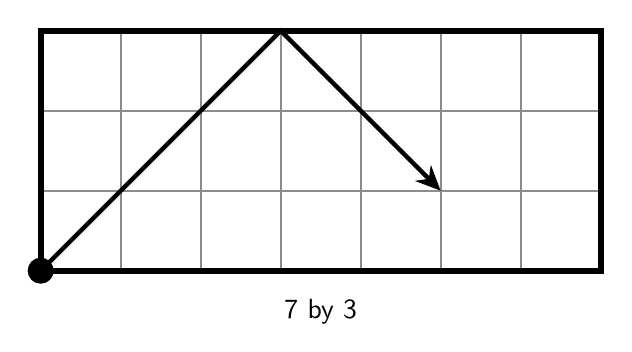
\begin{tikzpicture}[x=1in, y=1in]
\draw[black!45, line width=0.6pt] (0,0) -- (0,1.2);
\draw[black!45, line width=0.6pt] (0.4,0) -- (0.4,1.2);
\draw[black!45, line width=0.6pt] (0.8,0) -- (0.8,1.2);
\draw[black!45, line width=0.6pt] (1.2,0) -- (1.2,1.2);
\draw[black!45, line width=0.6pt] (1.6,0) -- (1.6,1.2);
\draw[black!45, line width=0.6pt] (2,0) -- (2,1.2);
\draw[black!45, line width=0.6pt] (2.4,0) -- (2.4,1.2);
\draw[black!45, line width=0.6pt] (2.8,0) -- (2.8,1.2);
\draw[black!45, line width=0.6pt] (0,0) -- (2.8,0);
\draw[black!45, line width=0.6pt] (0,0.4) -- (2.8,0.4);
\draw[black!45, line width=0.6pt] (0,0.8) -- (2.8,0.8);
\draw[black!45, line width=0.6pt] (0,1.2) -- (2.8,1.2);
\draw[line width=2.2pt] (0,0) rectangle (2.8,1.2);
\draw[line width=1.6pt, -{Stealth[length=9pt,width=8pt]}] (0,0) -- (0.4,0.4) -- (0.8,0.8) -- (1.2,1.2) -- (1.6,0.8) -- (2,0.4);
\fill (0,0) circle (0.065);
\node[anchor=north, inner sep=0pt] at (1.4,-0.14) {\normalsize 7 by 3};
\end{tikzpicture}
\end{minipage}

\vspace*{0.05in}
\prob{1} Trace the path on each table. Under each table, write the corner where the ball stops and the number of bounces.
\begin{center}
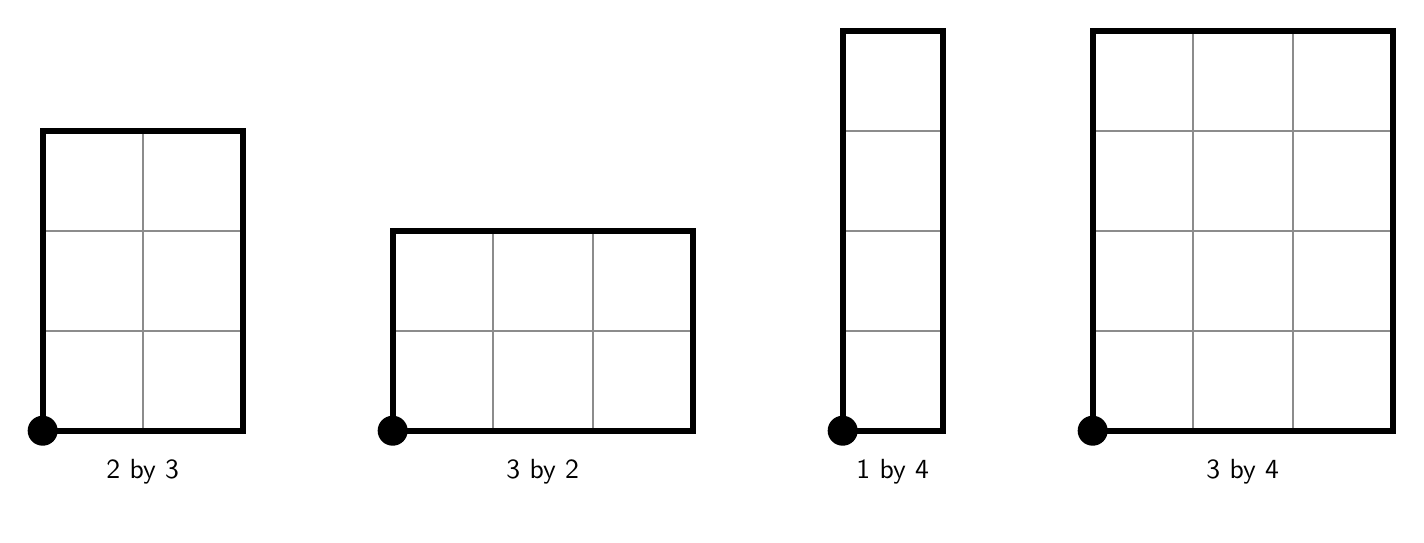
\begin{tikzpicture}[x=1in, y=1in]
\draw[black!45, line width=0.6pt] (0,0) -- (0,1.5);
\draw[black!45, line width=0.6pt] (0.5,0) -- (0.5,1.5);
\draw[black!45, line width=0.6pt] (1,0) -- (1,1.5);
\draw[black!45, line width=0.6pt] (0,0) -- (1,0);
\draw[black!45, line width=0.6pt] (0,0.5) -- (1,0.5);
\draw[black!45, line width=0.6pt] (0,1) -- (1,1);
\draw[black!45, line width=0.6pt] (0,1.5) -- (1,1.5);
\draw[line width=2.2pt] (0,0) rectangle (1,1.5);
\fill (0,0) circle (0.075);
\node[anchor=north, inner sep=0pt] at (0.5,-0.14) {\normalsize 2 by 3};
\draw[black!45, line width=0.6pt] (1.75,0) -- (1.75,1);
\draw[black!45, line width=0.6pt] (2.25,0) -- (2.25,1);
\draw[black!45, line width=0.6pt] (2.75,0) -- (2.75,1);
\draw[black!45, line width=0.6pt] (3.25,0) -- (3.25,1);
\draw[black!45, line width=0.6pt] (1.75,0) -- (3.25,0);
\draw[black!45, line width=0.6pt] (1.75,0.5) -- (3.25,0.5);
\draw[black!45, line width=0.6pt] (1.75,1) -- (3.25,1);
\draw[line width=2.2pt] (1.75,0) rectangle (3.25,1);
\fill (1.75,0) circle (0.075);
\node[anchor=north, inner sep=0pt] at (2.5,-0.14) {\normalsize 3 by 2};
\draw[black!45, line width=0.6pt] (4,0) -- (4,2);
\draw[black!45, line width=0.6pt] (4.5,0) -- (4.5,2);
\draw[black!45, line width=0.6pt] (4,0) -- (4.5,0);
\draw[black!45, line width=0.6pt] (4,0.5) -- (4.5,0.5);
\draw[black!45, line width=0.6pt] (4,1) -- (4.5,1);
\draw[black!45, line width=0.6pt] (4,1.5) -- (4.5,1.5);
\draw[black!45, line width=0.6pt] (4,2) -- (4.5,2);
\draw[line width=2.2pt] (4,0) rectangle (4.5,2);
\fill (4,0) circle (0.075);
\node[anchor=north, inner sep=0pt] at (4.25,-0.14) {\normalsize 1 by 4};
\draw[black!45, line width=0.6pt] (5.25,0) -- (5.25,2);
\draw[black!45, line width=0.6pt] (5.75,0) -- (5.75,2);
\draw[black!45, line width=0.6pt] (6.25,0) -- (6.25,2);
\draw[black!45, line width=0.6pt] (6.75,0) -- (6.75,2);
\draw[black!45, line width=0.6pt] (5.25,0) -- (6.75,0);
\draw[black!45, line width=0.6pt] (5.25,0.5) -- (6.75,0.5);
\draw[black!45, line width=0.6pt] (5.25,1) -- (6.75,1);
\draw[black!45, line width=0.6pt] (5.25,1.5) -- (6.75,1.5);
\draw[black!45, line width=0.6pt] (5.25,2) -- (6.75,2);
\draw[line width=2.2pt] (5.25,0) rectangle (6.75,2);
\fill (5.25,0) circle (0.075);
\node[anchor=north, inner sep=0pt] at (6,-0.14) {\normalsize 3 by 4};
\path (0,-0.42) rectangle (6.75,2);
\end{tikzpicture}
\end{center}
\vspace*{0.2in}
\begin{center}
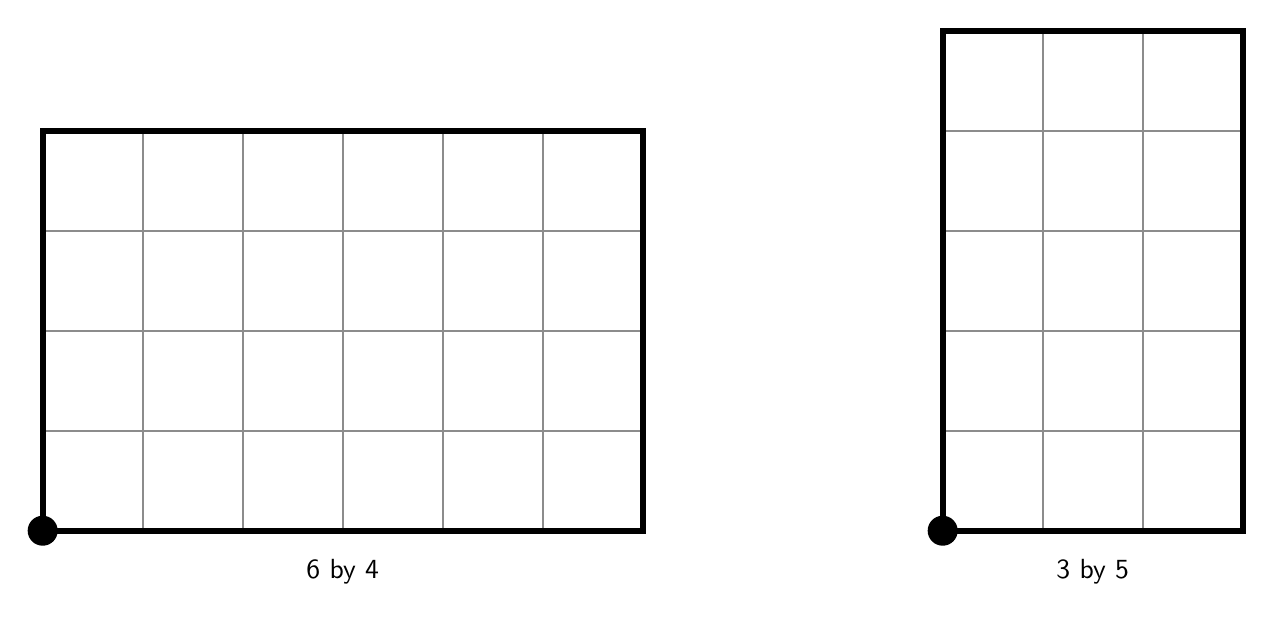
\begin{tikzpicture}[x=1in, y=1in]
\draw[black!45, line width=0.6pt] (0,0) -- (0,2);
\draw[black!45, line width=0.6pt] (0.5,0) -- (0.5,2);
\draw[black!45, line width=0.6pt] (1,0) -- (1,2);
\draw[black!45, line width=0.6pt] (1.5,0) -- (1.5,2);
\draw[black!45, line width=0.6pt] (2,0) -- (2,2);
\draw[black!45, line width=0.6pt] (2.5,0) -- (2.5,2);
\draw[black!45, line width=0.6pt] (3,0) -- (3,2);
\draw[black!45, line width=0.6pt] (0,0) -- (3,0);
\draw[black!45, line width=0.6pt] (0,0.5) -- (3,0.5);
\draw[black!45, line width=0.6pt] (0,1) -- (3,1);
\draw[black!45, line width=0.6pt] (0,1.5) -- (3,1.5);
\draw[black!45, line width=0.6pt] (0,2) -- (3,2);
\draw[line width=2.2pt] (0,0) rectangle (3,2);
\fill (0,0) circle (0.075);
\node[anchor=north, inner sep=0pt] at (1.5,-0.14) {\normalsize 6 by 4};
\draw[black!45, line width=0.6pt] (4.5,0) -- (4.5,2.5);
\draw[black!45, line width=0.6pt] (5,0) -- (5,2.5);
\draw[black!45, line width=0.6pt] (5.5,0) -- (5.5,2.5);
\draw[black!45, line width=0.6pt] (6,0) -- (6,2.5);
\draw[black!45, line width=0.6pt] (4.5,0) -- (6,0);
\draw[black!45, line width=0.6pt] (4.5,0.5) -- (6,0.5);
\draw[black!45, line width=0.6pt] (4.5,1) -- (6,1);
\draw[black!45, line width=0.6pt] (4.5,1.5) -- (6,1.5);
\draw[black!45, line width=0.6pt] (4.5,2) -- (6,2);
\draw[black!45, line width=0.6pt] (4.5,2.5) -- (6,2.5);
\draw[line width=2.2pt] (4.5,0) rectangle (6,2.5);
\fill (4.5,0) circle (0.075);
\node[anchor=north, inner sep=0pt] at (5.25,-0.14) {\normalsize 3 by 5};
\path (0,-0.42) rectangle (6,2.5);
\end{tikzpicture}
\end{center}
\newpage
\prob{2} Find where the ball stops and how many times it bounces on every table from 1 by 1 to 6 by 6. Record each table in the chart: put a dot in the corner of its box where the ball stops, and write the number of bounces inside the box.
\vspace*{0.2in}
\begin{center}
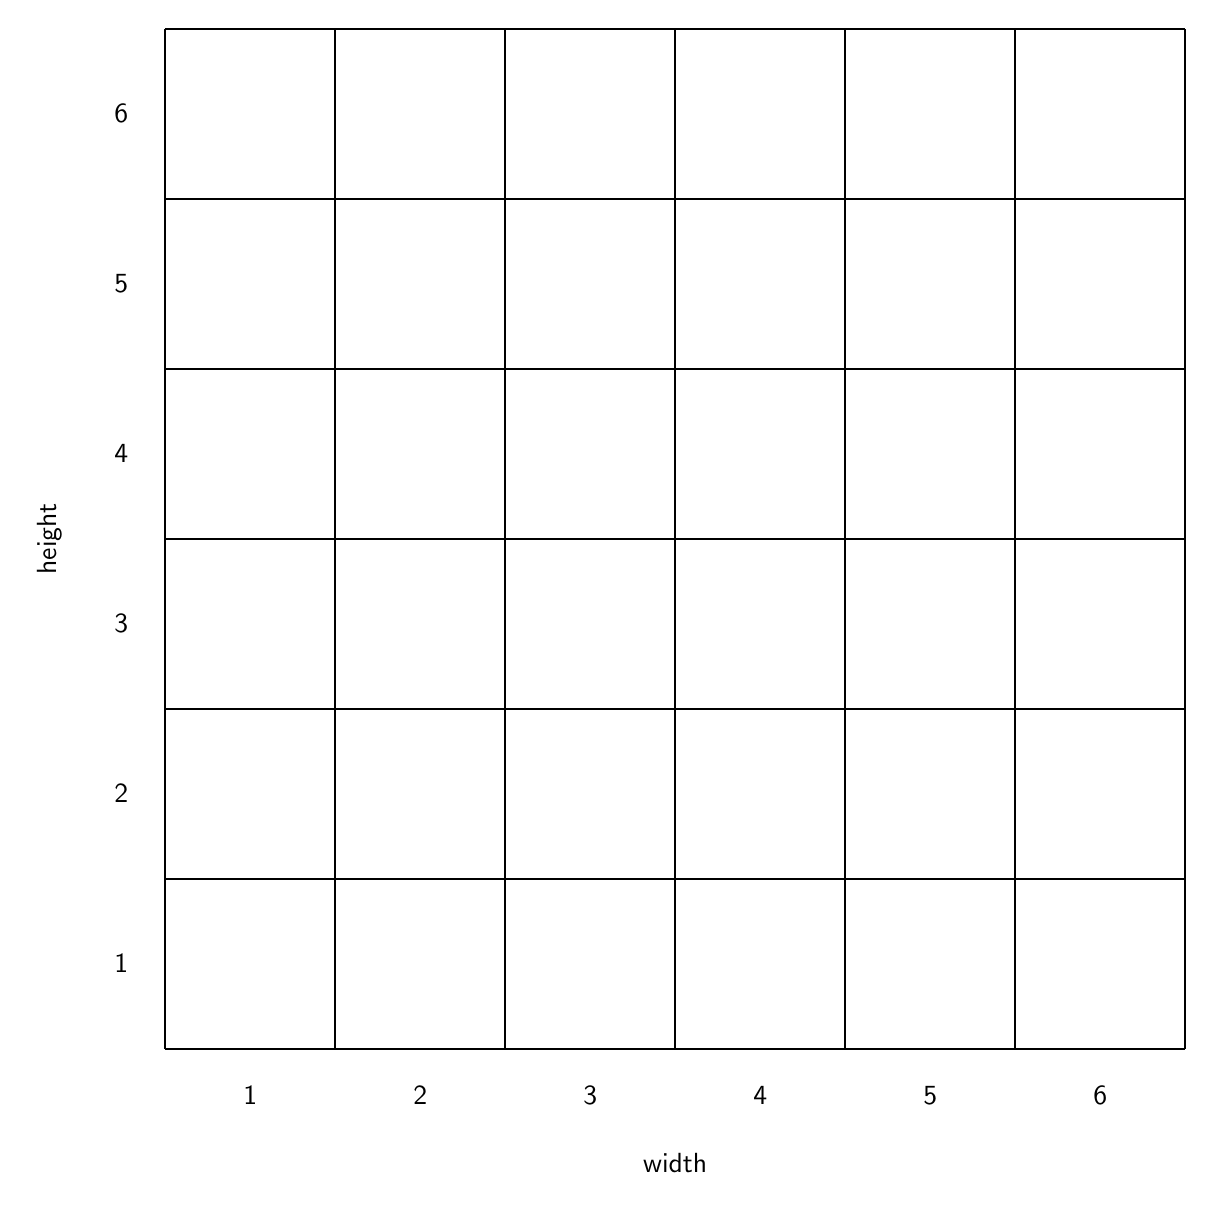
\begin{tikzpicture}[x=1in, y=1in]
\draw[line width=0.9pt] (0,0) -- (0,5.1);
\draw[line width=0.9pt] (0,0) -- (5.1,0);
\draw[line width=0.9pt] (0.85,0) -- (0.85,5.1);
\draw[line width=0.9pt] (0,0.85) -- (5.1,0.85);
\draw[line width=0.9pt] (1.7,0) -- (1.7,5.1);
\draw[line width=0.9pt] (0,1.7) -- (5.1,1.7);
\draw[line width=0.9pt] (2.55,0) -- (2.55,5.1);
\draw[line width=0.9pt] (0,2.55) -- (5.1,2.55);
\draw[line width=0.9pt] (3.4,0) -- (3.4,5.1);
\draw[line width=0.9pt] (0,3.4) -- (5.1,3.4);
\draw[line width=0.9pt] (4.25,0) -- (4.25,5.1);
\draw[line width=0.9pt] (0,4.25) -- (5.1,4.25);
\draw[line width=0.9pt] (5.1,0) -- (5.1,5.1);
\draw[line width=0.9pt] (0,5.1) -- (5.1,5.1);
\node[anchor=base] at (0.425,-0.28) {1};
\node at (-0.22,0.425) {1};
\node[anchor=base] at (1.275,-0.28) {2};
\node at (-0.22,1.275) {2};
\node[anchor=base] at (2.125,-0.28) {3};
\node at (-0.22,2.125) {3};
\node[anchor=base] at (2.975,-0.28) {4};
\node at (-0.22,2.975) {4};
\node[anchor=base] at (3.825,-0.28) {5};
\node at (-0.22,3.825) {5};
\node[anchor=base] at (4.675,-0.28) {6};
\node at (-0.22,4.675) {6};
\node[anchor=base] at (2.55,-0.62) {width};
\node[rotate=90] at (-0.58,2.55) {height};
\path (0,-0.75) rectangle (5.1,5.1);
\end{tikzpicture}
\end{center}
\newpage
\begin{center}
\begin{tikzpicture}[x=1in, y=1in]
\draw[black!45, line width=0.6pt] (0,0) -- (0,8);
\draw[black!45, line width=0.6pt] (0.5,0) -- (0.5,8);
\draw[black!45, line width=0.6pt] (1,0) -- (1,8);
\draw[black!45, line width=0.6pt] (1.5,0) -- (1.5,8);
\draw[black!45, line width=0.6pt] (2,0) -- (2,8);
\draw[black!45, line width=0.6pt] (2.5,0) -- (2.5,8);
\draw[black!45, line width=0.6pt] (3,0) -- (3,8);
\draw[black!45, line width=0.6pt] (3.5,0) -- (3.5,8);
\draw[black!45, line width=0.6pt] (4,0) -- (4,8);
\draw[black!45, line width=0.6pt] (4.5,0) -- (4.5,8);
\draw[black!45, line width=0.6pt] (5,0) -- (5,8);
\draw[black!45, line width=0.6pt] (5.5,0) -- (5.5,8);
\draw[black!45, line width=0.6pt] (6,0) -- (6,8);
\draw[black!45, line width=0.6pt] (6.5,0) -- (6.5,8);
\draw[black!45, line width=0.6pt] (7,0) -- (7,8);
\draw[black!45, line width=0.6pt] (0,0) -- (7,0);
\draw[black!45, line width=0.6pt] (0,0.5) -- (7,0.5);
\draw[black!45, line width=0.6pt] (0,1) -- (7,1);
\draw[black!45, line width=0.6pt] (0,1.5) -- (7,1.5);
\draw[black!45, line width=0.6pt] (0,2) -- (7,2);
\draw[black!45, line width=0.6pt] (0,2.5) -- (7,2.5);
\draw[black!45, line width=0.6pt] (0,3) -- (7,3);
\draw[black!45, line width=0.6pt] (0,3.5) -- (7,3.5);
\draw[black!45, line width=0.6pt] (0,4) -- (7,4);
\draw[black!45, line width=0.6pt] (0,4.5) -- (7,4.5);
\draw[black!45, line width=0.6pt] (0,5) -- (7,5);
\draw[black!45, line width=0.6pt] (0,5.5) -- (7,5.5);
\draw[black!45, line width=0.6pt] (0,6) -- (7,6);
\draw[black!45, line width=0.6pt] (0,6.5) -- (7,6.5);
\draw[black!45, line width=0.6pt] (0,7) -- (7,7);
\draw[black!45, line width=0.6pt] (0,7.5) -- (7,7.5);
\draw[black!45, line width=0.6pt] (0,8) -- (7,8);
\path (0,-0) rectangle (7,8);
\end{tikzpicture}
\end{center}
\newpage
\prob{3} With a ruler and a dark marker, draw a straight line on the big sheet from the dot, crossing each square from corner to corner. Stop when the line first reaches another point where two thick lines cross. How many thick lines did it cross before it reached that point? Then cut out the tables the line passes through, keeping them in one piece. Fold them on the thick lines until they are the size of the 2 by 3 table with the dot in front. Hold them up to the light, and copy the path you see onto the small 2 by 3 table.
\vspace*{0.15in}
\begin{center}
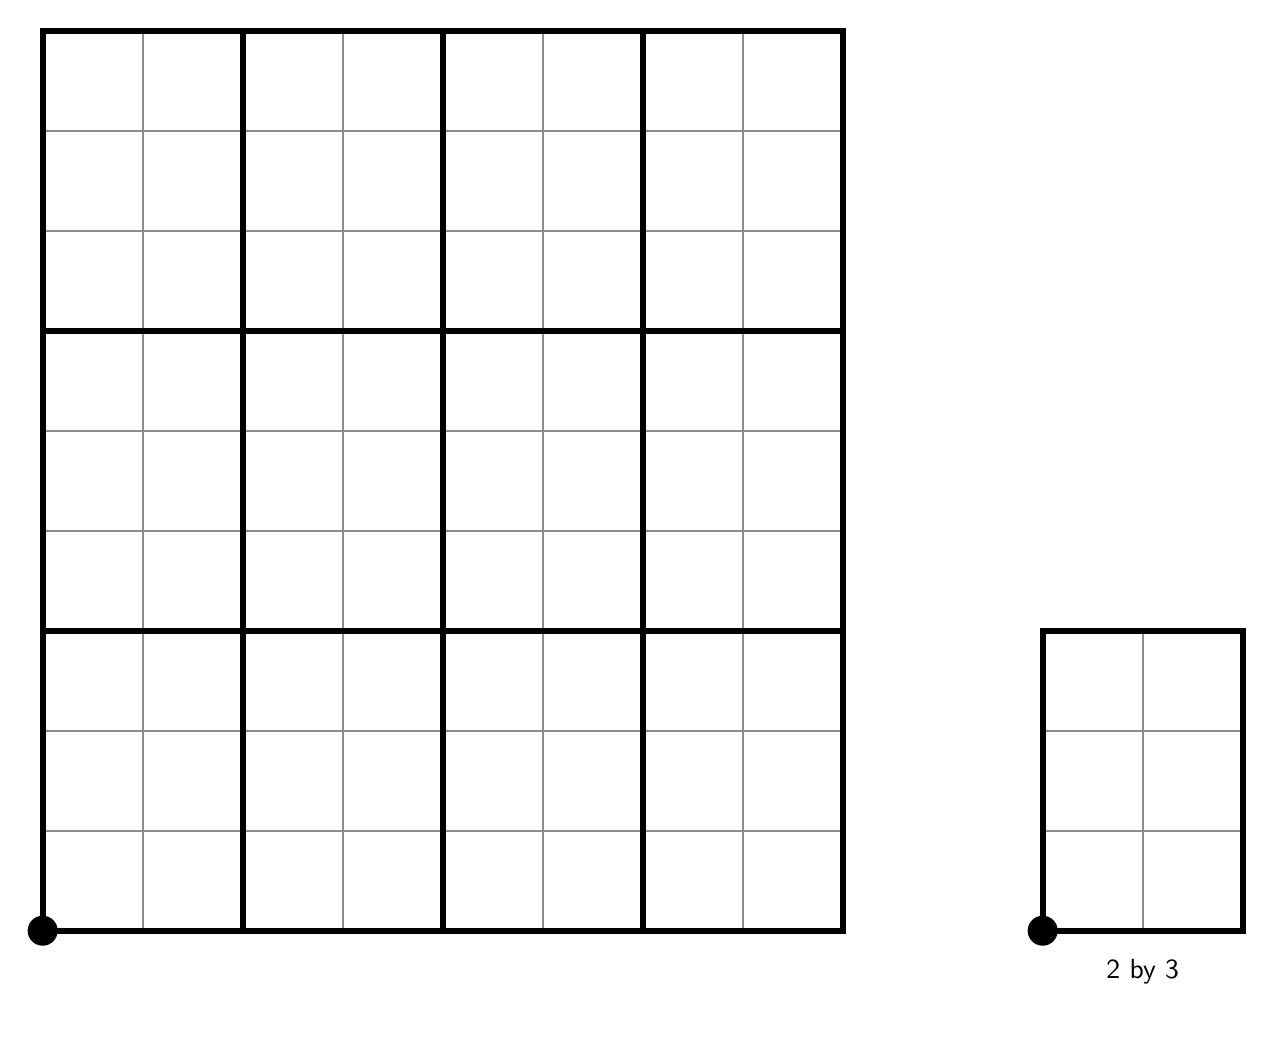
\begin{tikzpicture}[x=1in, y=1in]
\draw[black!45, line width=0.6pt] (0,0) -- (0,4.5);
\draw[black!45, line width=0.6pt] (0.5,0) -- (0.5,4.5);
\draw[black!45, line width=0.6pt] (1,0) -- (1,4.5);
\draw[black!45, line width=0.6pt] (1.5,0) -- (1.5,4.5);
\draw[black!45, line width=0.6pt] (2,0) -- (2,4.5);
\draw[black!45, line width=0.6pt] (2.5,0) -- (2.5,4.5);
\draw[black!45, line width=0.6pt] (3,0) -- (3,4.5);
\draw[black!45, line width=0.6pt] (3.5,0) -- (3.5,4.5);
\draw[black!45, line width=0.6pt] (4,0) -- (4,4.5);
\draw[black!45, line width=0.6pt] (0,0) -- (4,0);
\draw[black!45, line width=0.6pt] (0,0.5) -- (4,0.5);
\draw[black!45, line width=0.6pt] (0,1) -- (4,1);
\draw[black!45, line width=0.6pt] (0,1.5) -- (4,1.5);
\draw[black!45, line width=0.6pt] (0,2) -- (4,2);
\draw[black!45, line width=0.6pt] (0,2.5) -- (4,2.5);
\draw[black!45, line width=0.6pt] (0,3) -- (4,3);
\draw[black!45, line width=0.6pt] (0,3.5) -- (4,3.5);
\draw[black!45, line width=0.6pt] (0,4) -- (4,4);
\draw[black!45, line width=0.6pt] (0,4.5) -- (4,4.5);
\draw[line width=2.2pt] (1,0) -- (1,4.5);
\draw[line width=2.2pt] (2,0) -- (2,4.5);
\draw[line width=2.2pt] (3,0) -- (3,4.5);
\draw[line width=2.2pt] (0,1.5) -- (4,1.5);
\draw[line width=2.2pt] (0,3) -- (4,3);
\draw[line width=2.2pt] (0,0) rectangle (4,4.5);
\fill (0,0) circle (0.075);
\draw[black!45, line width=0.6pt] (5,0) -- (5,1.5);
\draw[black!45, line width=0.6pt] (5.5,0) -- (5.5,1.5);
\draw[black!45, line width=0.6pt] (6,0) -- (6,1.5);
\draw[black!45, line width=0.6pt] (5,0) -- (6,0);
\draw[black!45, line width=0.6pt] (5,0.5) -- (6,0.5);
\draw[black!45, line width=0.6pt] (5,1) -- (6,1);
\draw[black!45, line width=0.6pt] (5,1.5) -- (6,1.5);
\draw[line width=2.2pt] (5,0) rectangle (6,1.5);
\fill (5,0) circle (0.075);
\node[anchor=north, inner sep=0pt] at (5.5,-0.14) {\normalsize 2 by 3};
\path (0,-0.42) rectangle (6,4.5);
\end{tikzpicture}
\end{center}
\newpage
\prob{4} On this grid, draw thick lines to make a sheet for the 4 by 3 table, the way the sheet in Problem 3 is made for the 2 by 3 table. Draw the straight line from the dot until it first reaches another point where two thick lines cross. How many tables across and how many tables up does the line travel? Where does the ball stop on the 4 by 3 table, and how many times does it bounce?
\vspace*{0.05in}
\begin{center}

\begin{tikzpicture}[x=1in, y=1in]
\draw[black!45, line width=0.6pt] (0,0) -- (0,6.5);
\draw[black!45, line width=0.6pt] (0.5,0) -- (0.5,6.5);
\draw[black!45, line width=0.6pt] (1,0) -- (1,6.5);
\draw[black!45, line width=0.6pt] (1.5,0) -- (1.5,6.5);
\draw[black!45, line width=0.6pt] (2,0) -- (2,6.5);
\draw[black!45, line width=0.6pt] (2.5,0) -- (2.5,6.5);
\draw[black!45, line width=0.6pt] (3,0) -- (3,6.5);
\draw[black!45, line width=0.6pt] (3.5,0) -- (3.5,6.5);
\draw[black!45, line width=0.6pt] (4,0) -- (4,6.5);
\draw[black!45, line width=0.6pt] (4.5,0) -- (4.5,6.5);
\draw[black!45, line width=0.6pt] (5,0) -- (5,6.5);
\draw[black!45, line width=0.6pt] (5.5,0) -- (5.5,6.5);
\draw[black!45, line width=0.6pt] (6,0) -- (6,6.5);
\draw[black!45, line width=0.6pt] (6.5,0) -- (6.5,6.5);
\draw[black!45, line width=0.6pt] (0,0) -- (6.5,0);
\draw[black!45, line width=0.6pt] (0,0.5) -- (6.5,0.5);
\draw[black!45, line width=0.6pt] (0,1) -- (6.5,1);
\draw[black!45, line width=0.6pt] (0,1.5) -- (6.5,1.5);
\draw[black!45, line width=0.6pt] (0,2) -- (6.5,2);
\draw[black!45, line width=0.6pt] (0,2.5) -- (6.5,2.5);
\draw[black!45, line width=0.6pt] (0,3) -- (6.5,3);
\draw[black!45, line width=0.6pt] (0,3.5) -- (6.5,3.5);
\draw[black!45, line width=0.6pt] (0,4) -- (6.5,4);
\draw[black!45, line width=0.6pt] (0,4.5) -- (6.5,4.5);
\draw[black!45, line width=0.6pt] (0,5) -- (6.5,5);
\draw[black!45, line width=0.6pt] (0,5.5) -- (6.5,5.5);
\draw[black!45, line width=0.6pt] (0,6) -- (6.5,6);
\draw[black!45, line width=0.6pt] (0,6.5) -- (6.5,6.5);
\fill (0,0) circle (0.075);
\path (0,-0) rectangle (6.5,6.5);
\end{tikzpicture}
\end{center}
\newpage
\prob{5} Without tracing, find where the ball stops and how many times it bounces on each of these tables. Then trace the 6 by 10 table to check.
\vspace*{0.15in}
\par\noindent\begin{minipage}[t]{0.5\textwidth}\vspace{0pt}
{\renewcommand{\arraystretch}{2.7}\begin{tabular}{|>{\centering\arraybackslash}m{0.9in}|>{\centering\arraybackslash}m{1.25in}|>{\centering\arraybackslash}m{0.85in}|}\hline
table & corner & bounces \\\hline
6 by 10 & & \\\hline
8 by 12 & & \\\hline
12 by 9 & & \\\hline
7 by 5 & & \\\hline
5 by 8 & & \\\hline
20 by 30 & & \\\hline
\end{tabular}}
\end{minipage}\hfill\begin{minipage}[t]{0.45\textwidth}\vspace{0pt}\centering
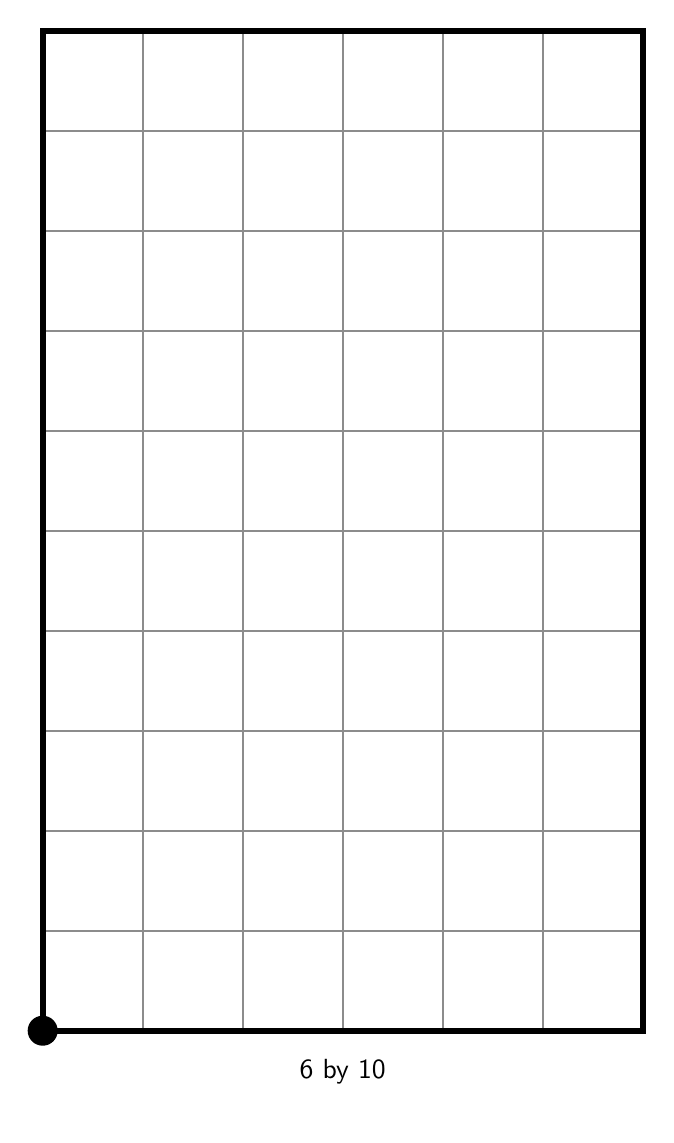
\begin{tikzpicture}[x=1in,y=1in]
\draw[black!45, line width=0.6pt] (0,0) -- (0,5);
\draw[black!45, line width=0.6pt] (0.5,0) -- (0.5,5);
\draw[black!45, line width=0.6pt] (1,0) -- (1,5);
\draw[black!45, line width=0.6pt] (1.5,0) -- (1.5,5);
\draw[black!45, line width=0.6pt] (2,0) -- (2,5);
\draw[black!45, line width=0.6pt] (2.5,0) -- (2.5,5);
\draw[black!45, line width=0.6pt] (3,0) -- (3,5);
\draw[black!45, line width=0.6pt] (0,0) -- (3,0);
\draw[black!45, line width=0.6pt] (0,0.5) -- (3,0.5);
\draw[black!45, line width=0.6pt] (0,1) -- (3,1);
\draw[black!45, line width=0.6pt] (0,1.5) -- (3,1.5);
\draw[black!45, line width=0.6pt] (0,2) -- (3,2);
\draw[black!45, line width=0.6pt] (0,2.5) -- (3,2.5);
\draw[black!45, line width=0.6pt] (0,3) -- (3,3);
\draw[black!45, line width=0.6pt] (0,3.5) -- (3,3.5);
\draw[black!45, line width=0.6pt] (0,4) -- (3,4);
\draw[black!45, line width=0.6pt] (0,4.5) -- (3,4.5);
\draw[black!45, line width=0.6pt] (0,5) -- (3,5);
\draw[line width=2.2pt] (0,0) rectangle (3,5);
\fill (0,0) circle (0.075);
\node[anchor=north, inner sep=0pt] at (1.5,-0.14) {\normalsize 6 by 10};
\path (0,-0.42) rectangle (3.0,5.0);
\end{tikzpicture}
\end{minipage}

\newpage
\prob{6} Find a table for each of these, or explain why there is none.
\begin{itemize}[itemsep=1pt, topsep=2pt]
\item The ball stops at the top left corner after 13 bounces.
\item The ball stops at the top right corner after 8 bounces.
\item The ball stops at the bottom right corner after 11 bounces.
\item The ball stops at the bottom right corner after 10 bounces.
\end{itemize}
\begin{center}
\begin{tikzpicture}[x=1in, y=1in]
\draw[black!45, line width=0.6pt] (0,0) -- (0,6);
\draw[black!45, line width=0.6pt] (0.5,0) -- (0.5,6);
\draw[black!45, line width=0.6pt] (1,0) -- (1,6);
\draw[black!45, line width=0.6pt] (1.5,0) -- (1.5,6);
\draw[black!45, line width=0.6pt] (2,0) -- (2,6);
\draw[black!45, line width=0.6pt] (2.5,0) -- (2.5,6);
\draw[black!45, line width=0.6pt] (3,0) -- (3,6);
\draw[black!45, line width=0.6pt] (3.5,0) -- (3.5,6);
\draw[black!45, line width=0.6pt] (4,0) -- (4,6);
\draw[black!45, line width=0.6pt] (4.5,0) -- (4.5,6);
\draw[black!45, line width=0.6pt] (5,0) -- (5,6);
\draw[black!45, line width=0.6pt] (5.5,0) -- (5.5,6);
\draw[black!45, line width=0.6pt] (6,0) -- (6,6);
\draw[black!45, line width=0.6pt] (6.5,0) -- (6.5,6);
\draw[black!45, line width=0.6pt] (7,0) -- (7,6);
\draw[black!45, line width=0.6pt] (0,0) -- (7,0);
\draw[black!45, line width=0.6pt] (0,0.5) -- (7,0.5);
\draw[black!45, line width=0.6pt] (0,1) -- (7,1);
\draw[black!45, line width=0.6pt] (0,1.5) -- (7,1.5);
\draw[black!45, line width=0.6pt] (0,2) -- (7,2);
\draw[black!45, line width=0.6pt] (0,2.5) -- (7,2.5);
\draw[black!45, line width=0.6pt] (0,3) -- (7,3);
\draw[black!45, line width=0.6pt] (0,3.5) -- (7,3.5);
\draw[black!45, line width=0.6pt] (0,4) -- (7,4);
\draw[black!45, line width=0.6pt] (0,4.5) -- (7,4.5);
\draw[black!45, line width=0.6pt] (0,5) -- (7,5);
\draw[black!45, line width=0.6pt] (0,5.5) -- (7,5.5);
\draw[black!45, line width=0.6pt] (0,6) -- (7,6);
\path (0,-0) rectangle (7,6);
\end{tikzpicture}
\end{center}
\newpage
\prob{7} Explain why the ball never stops at the corner where it started.
\vspace*{3.9in}

\prob{8} Write a rule that tells where the ball stops and how many times it bounces on any table, without tracing. Explain why your rule works.
\end{document}
